
\chapter{Thin Film Deposition}
After the detector sample has been mechanically processed and chemically polished, it is ready for the next steps of manufacturing: thin film deposition.
As mentioned in chapter 3, in order for the germanium detector to work, it must have the ability to block charge injection, low leakage current, and stability over time.
For these reasons and ease of manufacturing, amorphous germanium (AGe in short here after) is the chosen contact and passivation layer material at USD.
The AGe is deposited on the entire detector in two steps.
This is then followed by a deposition of aluminum on the top and bottom surfaces to provide good electrical contact to the detector.
After these metal layers are applied, the detector should be in working order.

\section{Amorphous Ge Deposition}

\subsection{Principles of Sputtering}
Sputter deposition is a method of thin film deposition that works well for AGe.
Sputtering works by ejecting atoms of a ``target'' material onto a substrate.
Figure \ref{fig:sput-theory} shows a graphic of the sputtering process.
The chamber is first vacuumed and then pressurized using a gas, usually argon.
Power is then transferred to the gas which is ionized. A plasma is then created.
The gas ions are then accelerated towards the target due to the electric field inside the chamber.
The ions bombard the target which then ejects neutral atoms which are deposited on the substrate and chamber walls.

\begin{figure}[htpb]
\centering
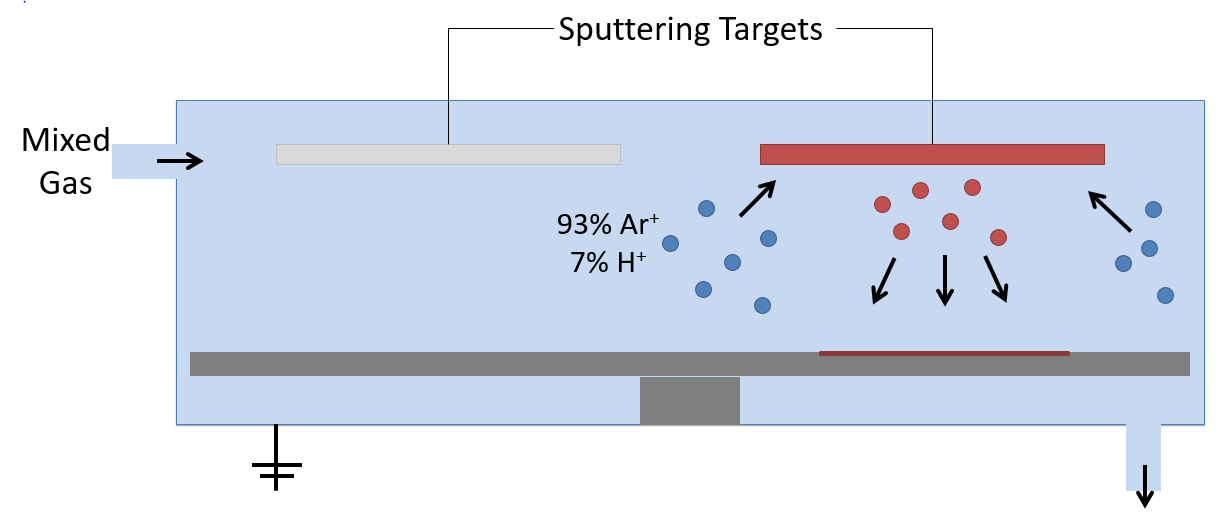
\includegraphics[width=0.8\textwidth]{sput-theory}
\caption{Schematics of the sputtering process.}
\label{fig:sput-theory}
\end{figure}

\subsection{Sputtering Calibration}
The AGe layer must achieve a minimum thickness in order to operate correctly.
Thus it is necessary to evaluate how much AGe is deposited during normal operating procedure with typical settings that would be used during detector fabrication.
The sputtering thickness is a function of time, distance from the target, gas pressure, and RF power.
The gas pressure of 14 mTorr has been found to be optimal and the sputtering machine at USD can generate a good plasma at this pressure with 100 watts of RF power.
Thus the only variables remaining are the amount of time sputtering and the position of the sample inside the machine.

To find out the optimal sputtering length and position, an experiment involving clean glass slides was implemented.
The idea is to block off a portion of the slide using tape and then to measure the step from the AGe region to the taped section.
The experiment was set up as shown in Figure \ref{fig:tape-test-s} using five glass slides in a cross shape centered under the germanium target.
The sputtering stage was set to the lowest position meaning that it was as far away from the target as possible.
The samples were then sputtered for 15 total minutes using a pressure of 14 mTorr and 100 watts of power.
\begin{figure}[htpb]
\centering
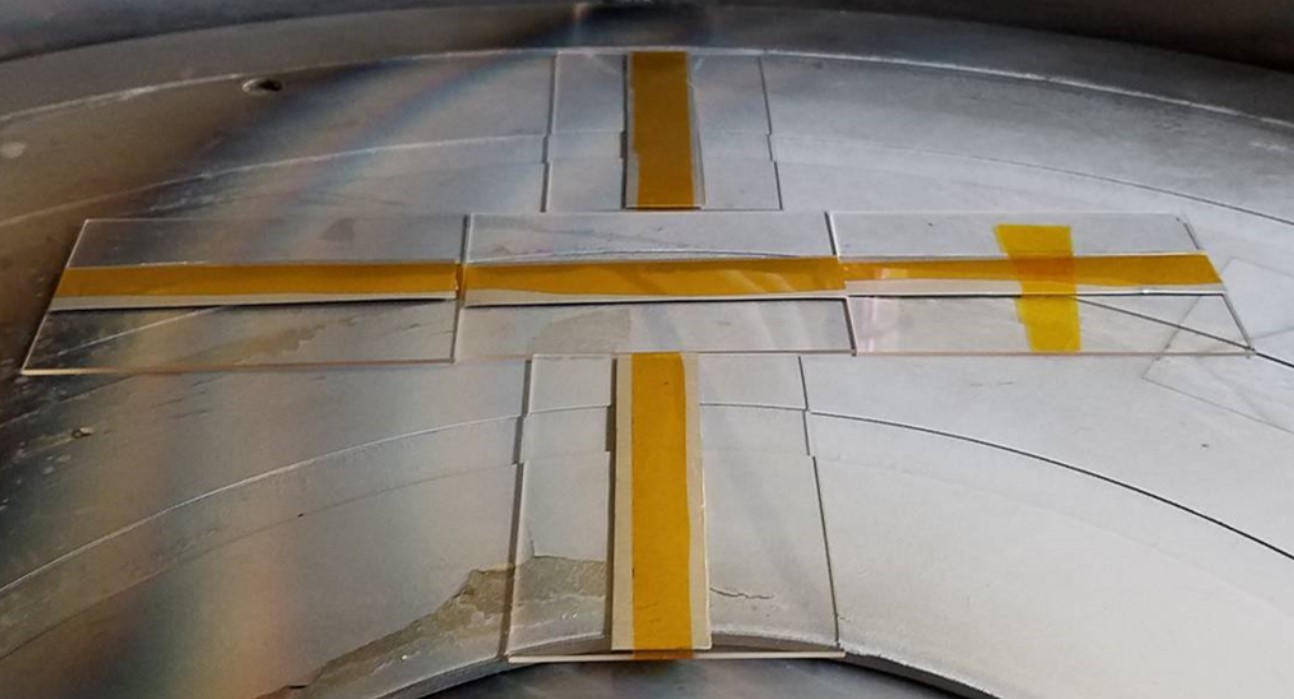
\includegraphics[width=0.5\textwidth]{tape-test-s}
\caption{Layout of tape test. Colors on the axis are exact, in between is linear interpolation.}
\label{fig:tape-test-s}
\end{figure}

Afterwords, the samples were removed from the sputtering machine and the tape was peeled off leaving a portion of the slide untouched by the deposition.
A machine called the Alpha-Step Profiler was used to measure the thickness of the deposited layer.
The profiler works by running a needle a predefined length across the surface.
Then it is possible to go from AGe region to the clean layer and measure the step down and thus the thickness of the deposited layer.
Figure \ref{fig:surface-prof} shows a plot of the thickness measured across the samples.
From this measurement, we learned that in the circle with a radius of about 4~cm, the deposition thickness is above 300~nm, which is enough for our purpose.
\begin{figure}[htpb]
\centering
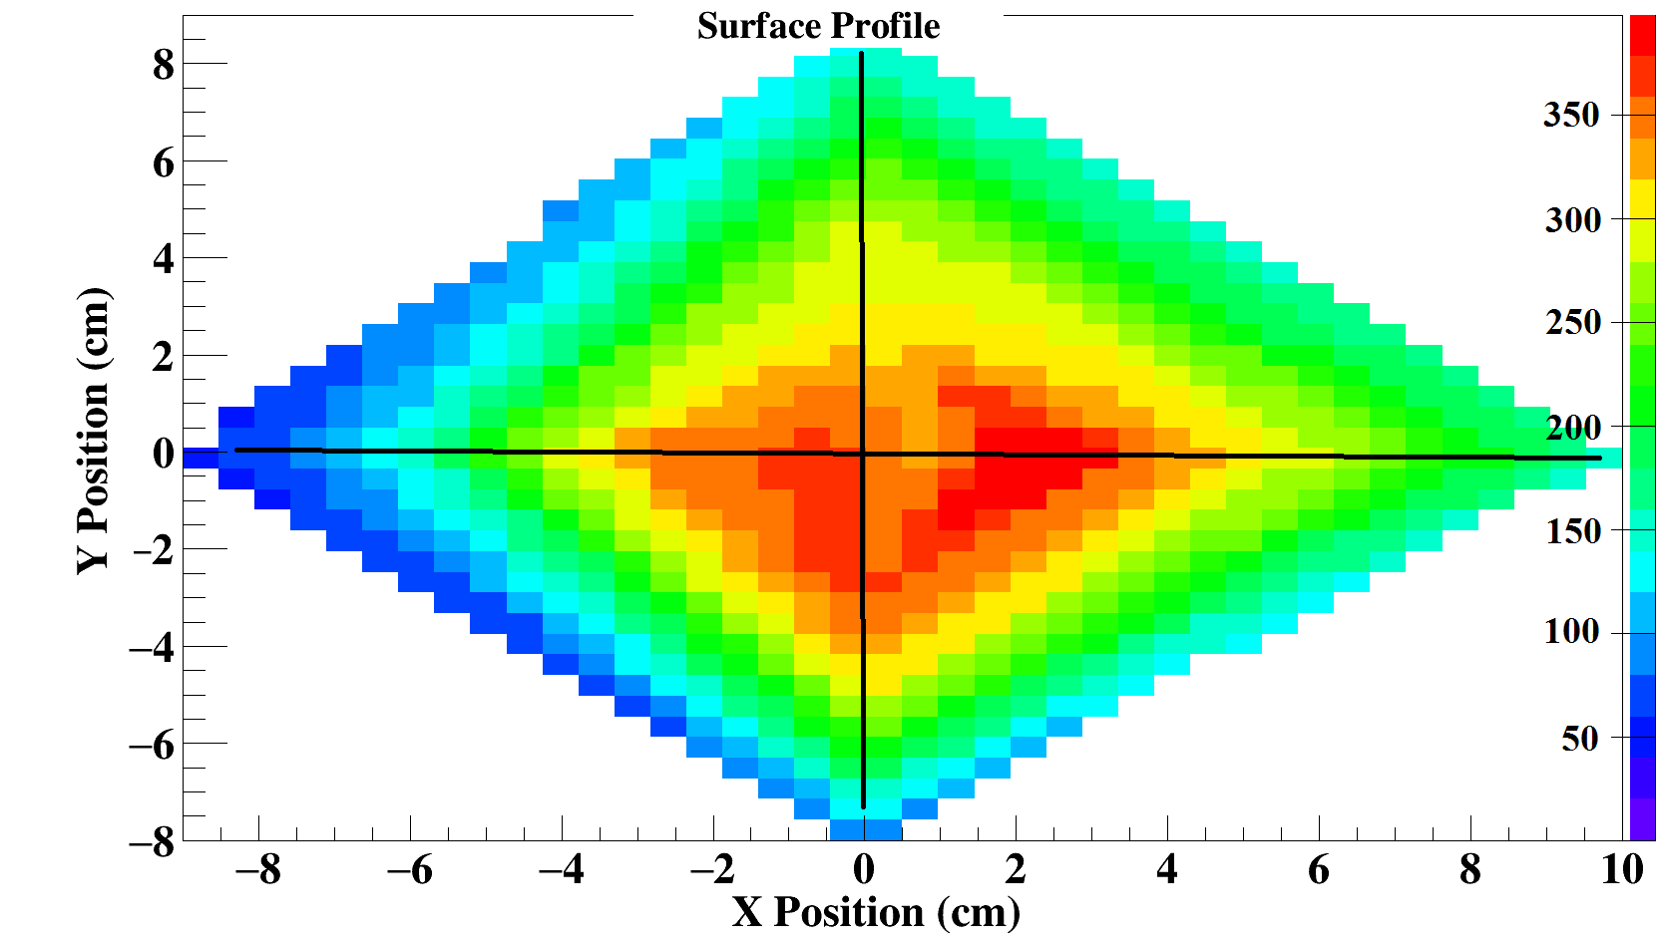
\includegraphics[width=0.8\textwidth]{surface-prof}
\caption{results of surface scan}
\label{fig:surface-prof}
\end{figure}

\subsection{Operating Procedure}
The sputtering machine at USD is a Perkin-Elmer 4400 Sputtering System.

The operating procedure for the sputtering machine is complex and care is required to make sure the system maintains working order.
It is a complex system with multiple valves, controls, power supplies, vacuum systems, and pressure monitors that all work in conjunction to deposit a thin layer of AGe on the detector sample.
One key component of the system is a cryopump that uses pressurized helium gas to quickly vacuum the system to the proper pressure.
The cryopump system can be seen in Figure ~\ref{fig:sput-flow} as blue boxes with labels connected by green lines.
The green lines exchange the helium between the cold head connected to the vacuum chamber and the compressor located in a separated pump room.
Before the sputtering procedure can begin, the cryopump must be turned on to allow the cold head to cool from room temperature to approximately 20K.
Prior to cooling down the cryopump, it must be vacuumed to below 100 mTorr using the rough pump described later.
In order to vacuum the cryopump, open the foreline valve shown as E in ~\ref{fig:sput-flow}; close the valve before turning on the cryopump.
The on/off switch for the compressor is located on the panel with the other valve toggles and is labeled as "HY-VAC PUMP".

\begin{sidewaysfigure}
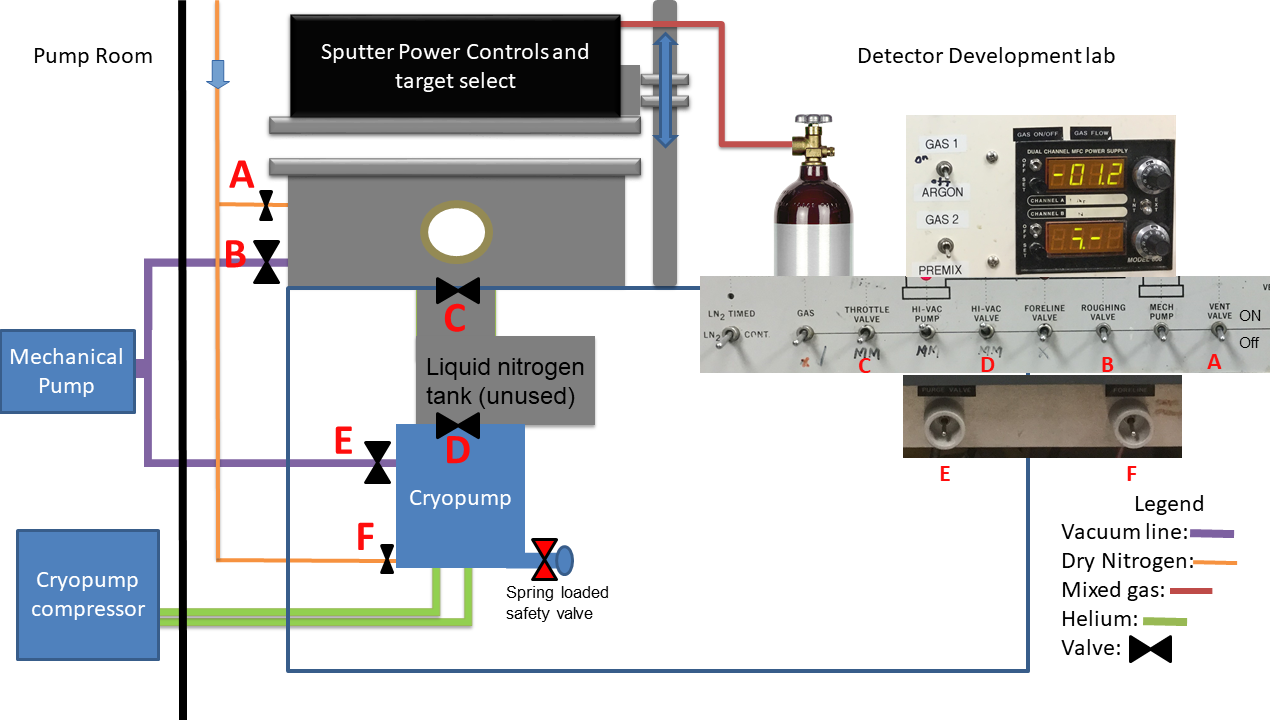
\includegraphics[width=\textwidth]{sput-flow}
\caption{This is a diagram of the Sputtering machine vacuum and gas system. Each valve is connected to a pressurized air line.}
\label{fig:sput-flow}
\end{sidewaysfigure}

Once the cryopump is cooled down to the proper temperature, the sputtering procedure can begin.
As seen in Figure ~\ref{fig:sput-flow}, there are multiple valves for opening and closing various gas and vacuum lines.
These valves are all pneumatically opened and closed. They require a constant supply of pressurized air at 60 psi.
This pressurized air is supplied by a large Kaeser SX 5 compressor located in the pump room and shown in Figure ~\ref{fig:comp-air}.
\begin{figure}[htpb]
\centering
\includegraphics[width=\textwidth]{comp-air}
\caption{Kaeser SX 5 compressor.}
\label{fig:comp-air}
\end{figure}
The compressor is turned on or off by pressing the green or red button on the control interface shown on the top left side of the figure.
Once turned on, it will automatically increase in pressure until it reaches a set point around 100 psi.
The pressure out is then reduced or increased by adjusting the pressure regulator shown on the bottom left.
It is important to check the pressure often to make sure that it is sufficiently high for if it drops too low, valves will return to the default closed position.

Once the system has been supplied with pressurized air, the valves can be opened or closed and the system is ready to be operated.
The next step is to load the detector sample into the sputtering machine and prepare for deposition.
The sputtering system should always be kept under vacuum so before it can be opened it must be returned to standard atmospheric pressure.
This is done by opening the vent valve and filling the chamber with dry nitrogen.
The toggle switch for the vent valve is located at 'A' in Figure ~\ref{fig:sput-flow}.
The nitrogen in routed in from a tank located in a separate room behind the pump room and is kept at approximately 10 to 15 psi.

After the chamber has returned to atmospheric pressure it can be opened using a hydraulic lift system that is powered through the RF power generator.
The sample can now be carefully placed inside the chamber centering it under the germanium target as seen in Figure ~\ref{fig:sput-open}.
\begin{figure}[htpb]
\centering
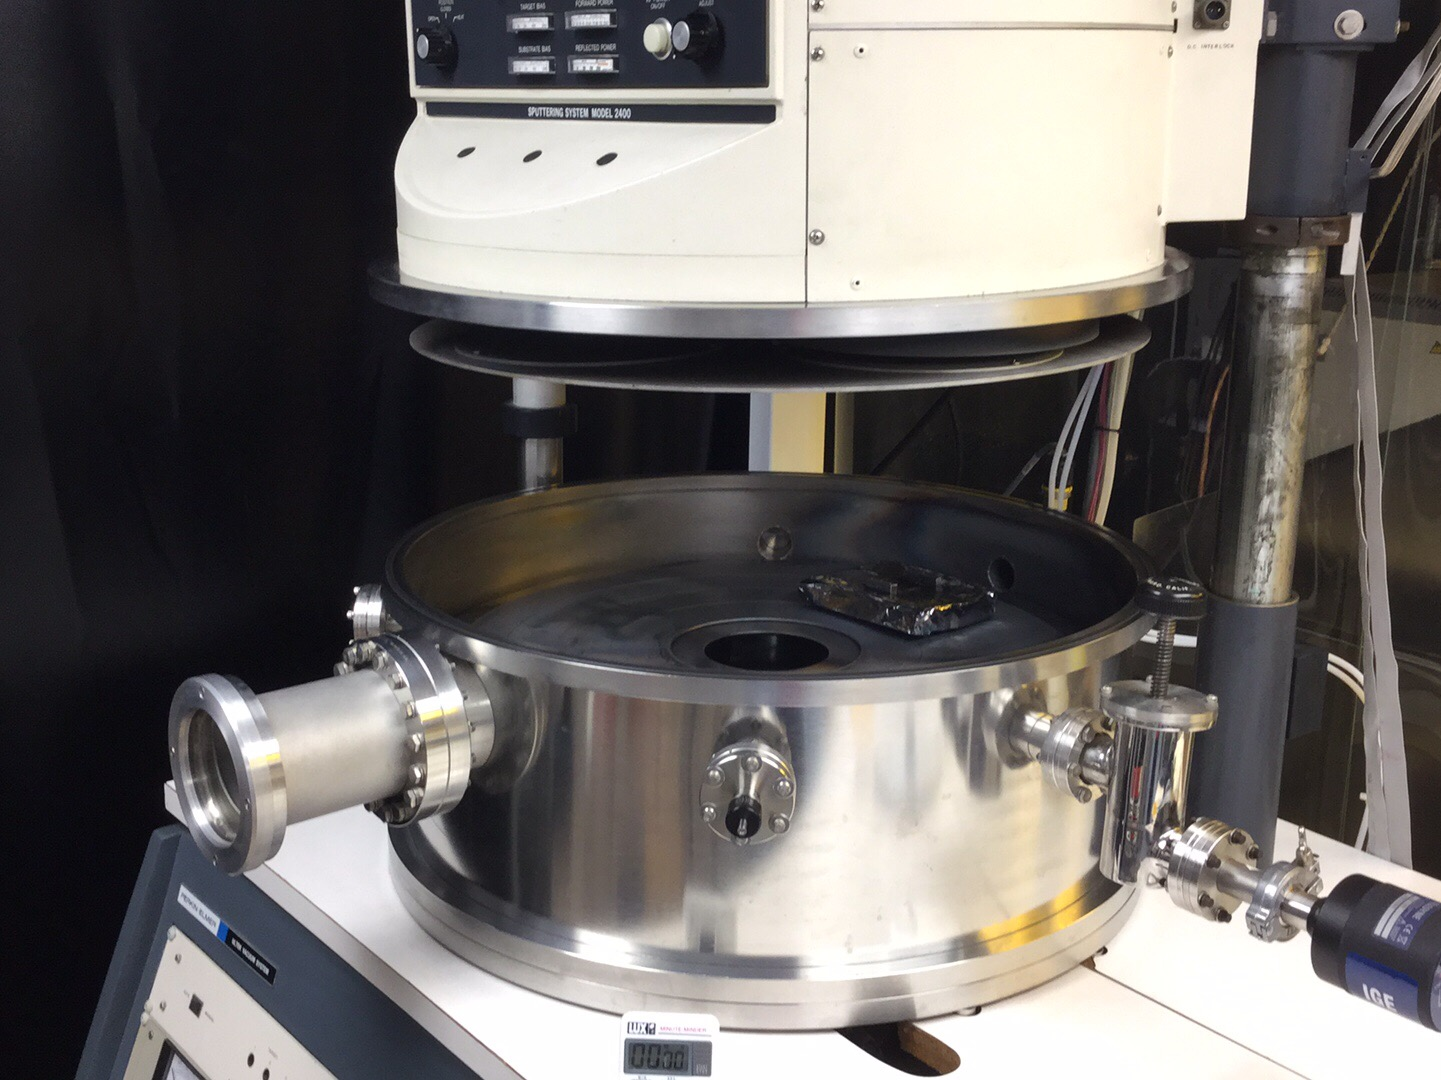
\includegraphics[width=0.6\textwidth]{sput-open}
\caption{Sputtering machine with chamber open.}
\label{fig:sput-open}
\end{figure}
A jig is used to hold the detectors by the wings during the sputtering process.
It is designed to be adjustable, allowing for various detector sizes and geometries.
After the detector sample has been chemically etched it can be loaded onto the jig and then into the sputtering machine.

Once the sample is loaded the chamber can be closed and vacuum pumping can begin.
The first stage of pumping is done by a rough pump which takes the chamber from atmospheric pressure down to below 100 mTorr.
The rough pump is turned on or off by switching an electrical breaker located outside of the clean room.
After the pump is on and running normally, the roughing valve can be opened.
Opening the roughing valve allows the rough pump to vacuum the chamber from atmospheric pressure to around 100 mTorr.

Once the chamber has reached some pressure between 50-100 mTorr the roughing valve can be closed and the HY-VAC VALVE, shown as D in Figure \ref{fig:sput-flow}, can be opened.
The cryopump will then be able to vacuum the system to the required $10^{-6}$ Torr for sputtering.
The sputtering machine takes less than five minutes to go from atmosphere to $10^{-3}$ Torr using the rough pump and a further 2-3 hours to reach $10^{-6}$ Torr using the cryopump.

After proper vacuum pressure is achieved the sputtering deposition procedure can start.
The first thing is to start the water chiller and make sure the proper lines are selected.
The chiller is used to provide cooling to the target and stage during deposition as the plasma generates considerable heat.
It is located in the pump room and is show in Figure ~\ref{fig:water-cool}.
The middle picture of the figure shows the side view of the chiller where the separate lines to the sputtering and e-beam machines are visible.
The selection of lines is done by switching two valves on the back of the water chiller.
The handles of the valves indicate the direction of flow and is used to determine which line is selected.
\begin{figure}[htpb]
\centering
\includegraphics[width=\textwidth]{water-cool}
\caption{Water chiller for cooling the sputtering machine and e-beam evaporator}
\label{fig:water-cool}
\end{figure}

Once the water chiller has reached the set point temperature of \SI{10}{\celsius}, the deposition can start.
First the RF power supply should be turned on by flipping the switch at the base of the front.
The throttle valve, shown as C in Figure ~\ref{fig:sput-flow}, can now be turned on to limit the vacuuming of the chamber.
Now the mixed gas can be vented into the chamber using the gas flow adjuster show in the figure.
To the left of the flow controller is the toggle switch to open the mixed gas line.
Then, the flow controller is turned on and set to approximately 50 SCCM.
Due to the throttle valve being on, the chamber will begin to increase in pressure based on the flow controller setting.
The key is to adjust the flow rate until a steady 14 mTorr chamber pressure is achieved.

After the chamber has stabilized at 14 mTorr the RF power can be introduced to the gas in order to generate the plasma required for sputtering.
This is done by pressing the power on button at the top of the chamber show in Figure.
The power can then slowly be increased to the marked point.
During this increase in power, the tune and load must be adjusted to keep the reflected power to a minimum and make sure all the power is transferred into the gas.
At a certain point, the plasma will form and the reading for forward and reflected power will jump up.
It is again necessary to quickly readjust the tune and load to get the reflected power back to 0.
After the reflected power is reduced, the power can be further adjusted to the required level, usually around 100 watts.
Once the plasma is generated, the user must wait for at least five minutes with the shutter closed to bombard the target and clean off the outer layer.
After this five minutes the shutter can be opened which will start deposition on the sample.
The machine can then be run for 15 minutes with the shutter open.
After 15 minutes have elapsed, the RF power can be turned off.
The detector sample should have accumulated a layer of AGe that is around 300 nm thick.

The machine can then be opened up and the sample flipped over to coat the other side.
This is done by first turning down the flow rate of the mixed gas to zero and closing the valve.
Then the throttle valve can be turned off followed by closing the HY-VAC VALVE.
At this point the chamber should no longer be pumping so the vent valve can be opened and the chamber returned to atmospheric pressure.
The sample can then be flipped and the sputtering process starts again with closing the chamber and rough pumping.



\section{Aluminum Deposition}
\subsection{Principles of e-beam}
\begin{figure}[htpb]
\centering
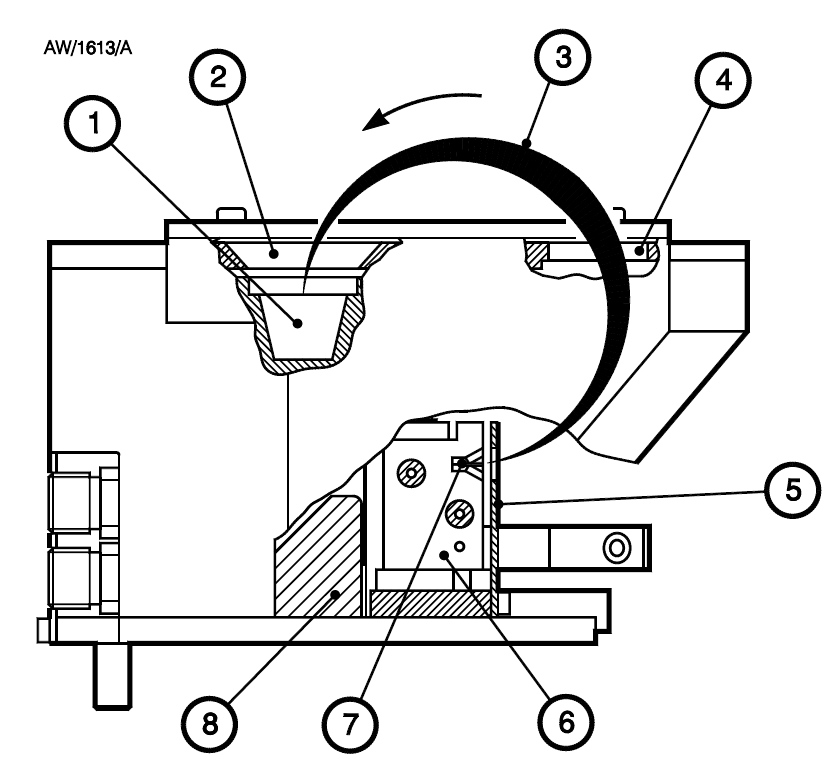
\includegraphics[width=0.6\textwidth]{ebeam-diagram}
\caption{Cutaway drawing of the e-beam mechanics. 1) crucible filled with aluminum, 3) electron beam, 4) field shaping magnets, 7) electron beam filament}
\label{fig:ebeam-diagram}
\end{figure}
Electron-beam deposition is a method of thin film deposition where a target metal is bombarded with an electron beam given off by a tungsten filament.
The electron beam then causes the atoms to transform into the gaseous phase which coats and solidifies onto everything within line of site of the material.
In order for e-beam deposition to work, the chamber must also be kept under high vacuum to make sure the electrons can make it from the gun to the crucible without interference.

\subsection{E-Beam Calibration}
The calibration of the e-beam was similar to the sputtering machine with a key difference being that the target location for the sample is fixed.
Due to this, only one glass slide was needed to get a good profile of the deposition thickness.
Another difference from the sputtering machine is that the e-beam has a deposition rate and thickness monitor.
Thus the accuracy of the monitor was also verified in the test.
\begin{table}[htpb]
\centering
\begin{tabular}{ |p{4cm}|p{4cm}|p{4cm}|  }
 \hline
 \multicolumn{3}{|c|}{E-Beam deposition profile} \\
 \hline
 Test (\#)&Step Thickness (nm)&Percent Difference (\%)\\
 \hline
 1   & 268.7    &7.48\\
 2&   256.7  & 2.68\\
 3 &268.1 & 7.24\\
 4    &246.2 & 1.52\\
 \hline
\end{tabular}
\caption{Table listing data gathered from alpha profiler}
\label{table:test-e}
\end{table}

Figure \ref{fig:tape-test-e} shows the glass slide after aluminum deposition.
Figure \ref{fig:alpha-step-e} shows a plot of thickness vs distance generated by the alpha step profiler.
In it, the step from an area with aluminum to one without is clearly visible.

\begin{figure}[htpb]
\centering
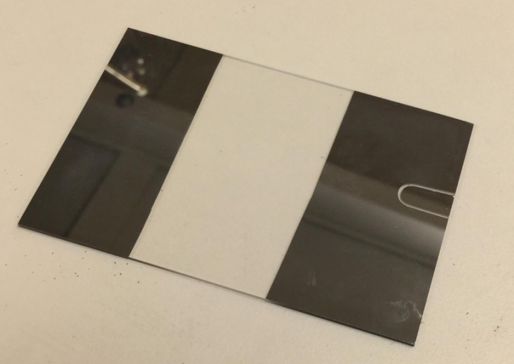
\includegraphics[width=0.5\textwidth]{tape-test-e}
\caption{E-Beam tape test}
\label{fig:tape-test-e}
\end{figure}

\begin{figure}[htpb]
\centering
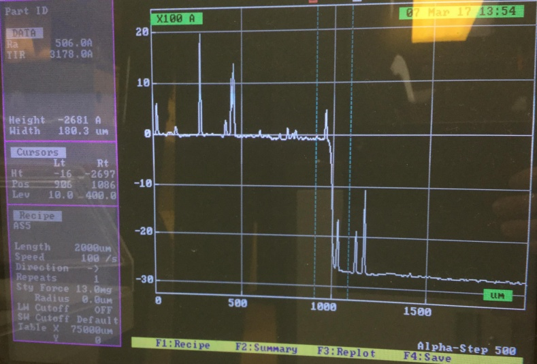
\includegraphics[width=0.7\textwidth]{alpha-step-e}
\caption{Surface profile for e-beam}
\label{fig:alpha-step-e}
\end{figure}

\subsection{Operating Procedure}
Once the detector sample has been completely coated with a layer of AGe, aluminum can be deposited on the top and bottom surface to create the electrical contacts.
The aluminum serves as the electrical contact and covers the entire surface of the top and bottom which is what defines the detector as planar.

The e-beam has two separate power supplies: one for powering the controls and vacuum system, and another for supplying the high voltage to the electron gun.
To initiate the startup procedure, the control power supply is turned on.
Afterwords the controls can be activated by switching the selector from 0 to 1 as seen in Figure \ref{fig:vac-control}.
This will supply power to the vacuum system which needs to be activated by following the prompts on the screen.
Pressing start will initialize the system, activating the rough and turbo pump.
Once the turbo pump has reached 42 krpm it is ready to vacuum.
\begin{figure}[htpb]
\centering
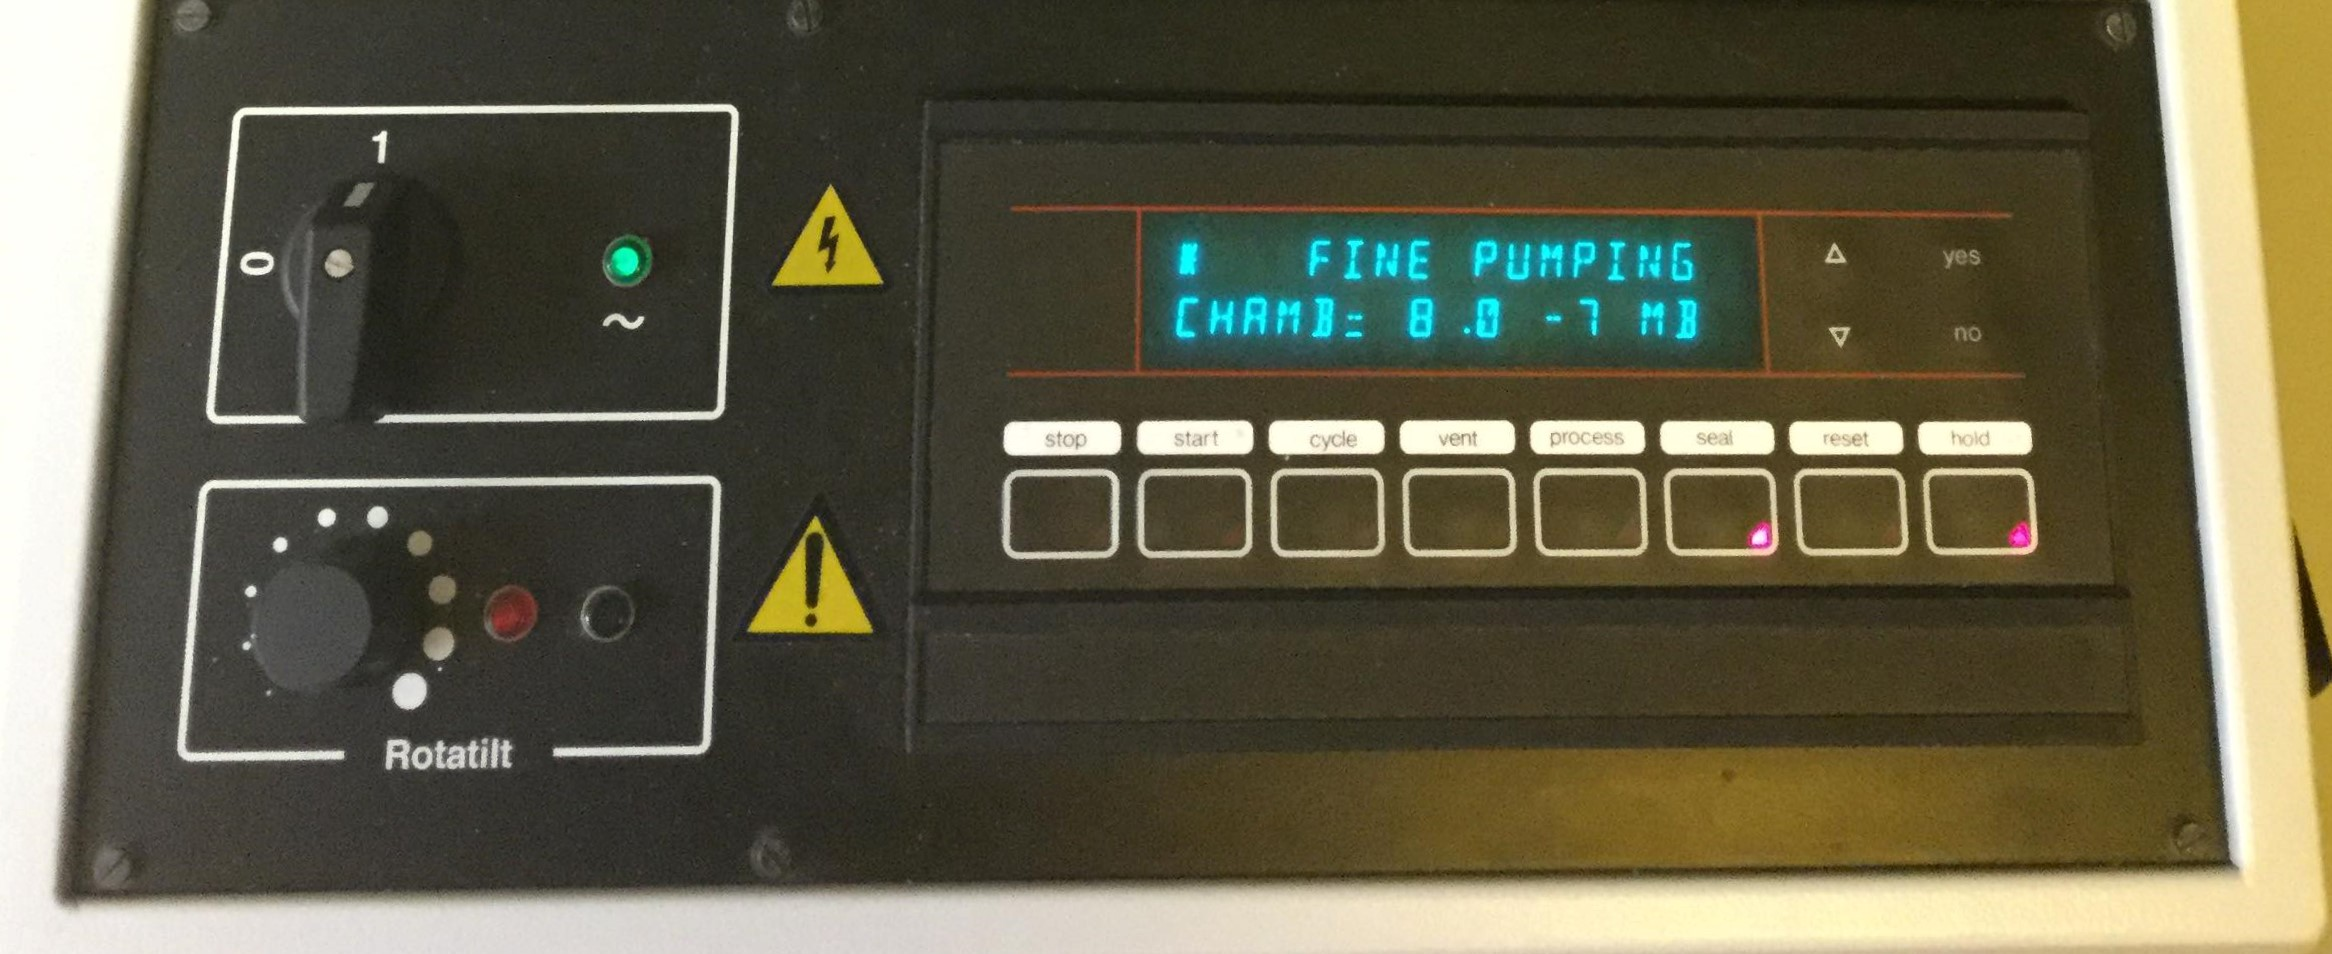
\includegraphics[width=\textwidth]{vac-control}
\caption{E-Beam vacuum controls and power switch}
\label{fig:vac-control}
\end{figure}

The vacuum pumps are located in a cabinet directly under the e-beam chamber as shown in Figure \ref{fig:ebeam-flow}.
The turbo pump has a separate controller that displays the speed which can be seen when the cabinet is opened.
Pressing seal will isolate the turbo pump from the chamber and allow it to be vented so the sample can be placed inside.
Once sealed, the vent button can be pressed which will open the valve allowing nitrogen to fill the chamber.
After the chamber has reached atmospheric pressure the door will be able to open and the sample can be placed loaded onto the holder shown in Figure \ref{fig:ebeam-holder}.
The holder can then be secured inside the chamber using a hex screw and wrench.
\begin{figure}[htpb]
\centering
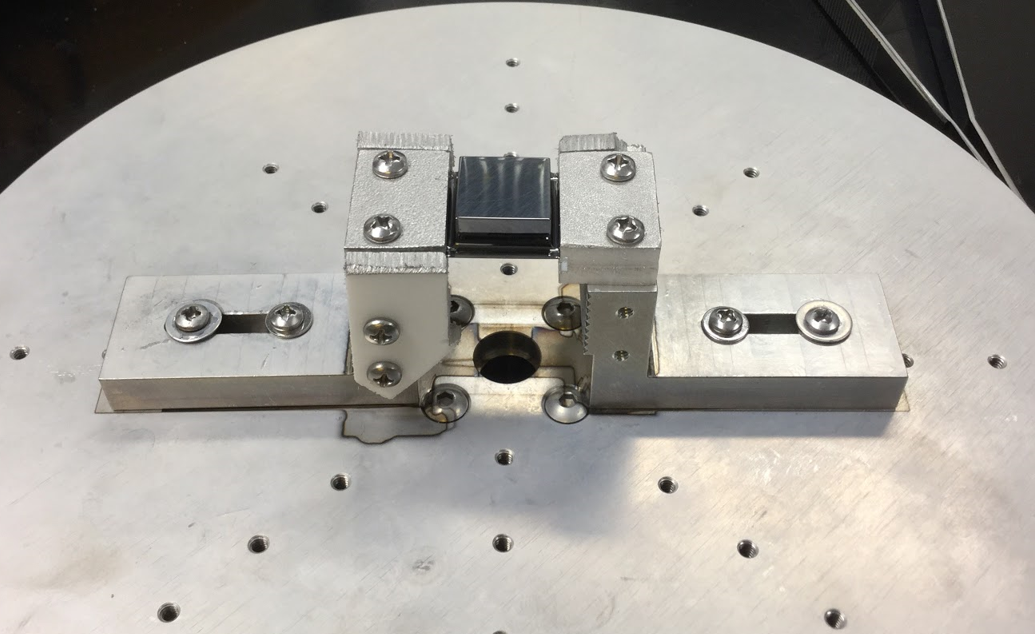
\includegraphics[width=0.6\textwidth]{ebeam-holder}
\caption{Sample holder for the E-Beam}
\label{fig:ebeam-holder}
\end{figure}
Once the sample is loaded, the chamber door can be closed and the process button pressed.
This will open up the chamber to the vacuum system and start the rough pump.
Once the vacuum has reached sufficient level, the turbo pump will automatically turn on.
The vacuum must reach around $10^{-6}$ torr before the aluminum deposition can start.

Once the proper pressure is reached, the aluminum deposition can begin.
To start, the electron gun power supply is turned on by flipping the switch on the front panel of the high voltage power supply.
Then the on/off switch on the source control, shown in the upper right of Figure \ref{fig:source-control}, can be switched on.
The gun button can then be depressed.
This will provide around 4.9 kV to the electron gun, however, the current remains at 0 so there is no flow of electrons yet.
The current can then be turned up slowly using the dial labeled current.
\begin{figure}[htpb]
\centering
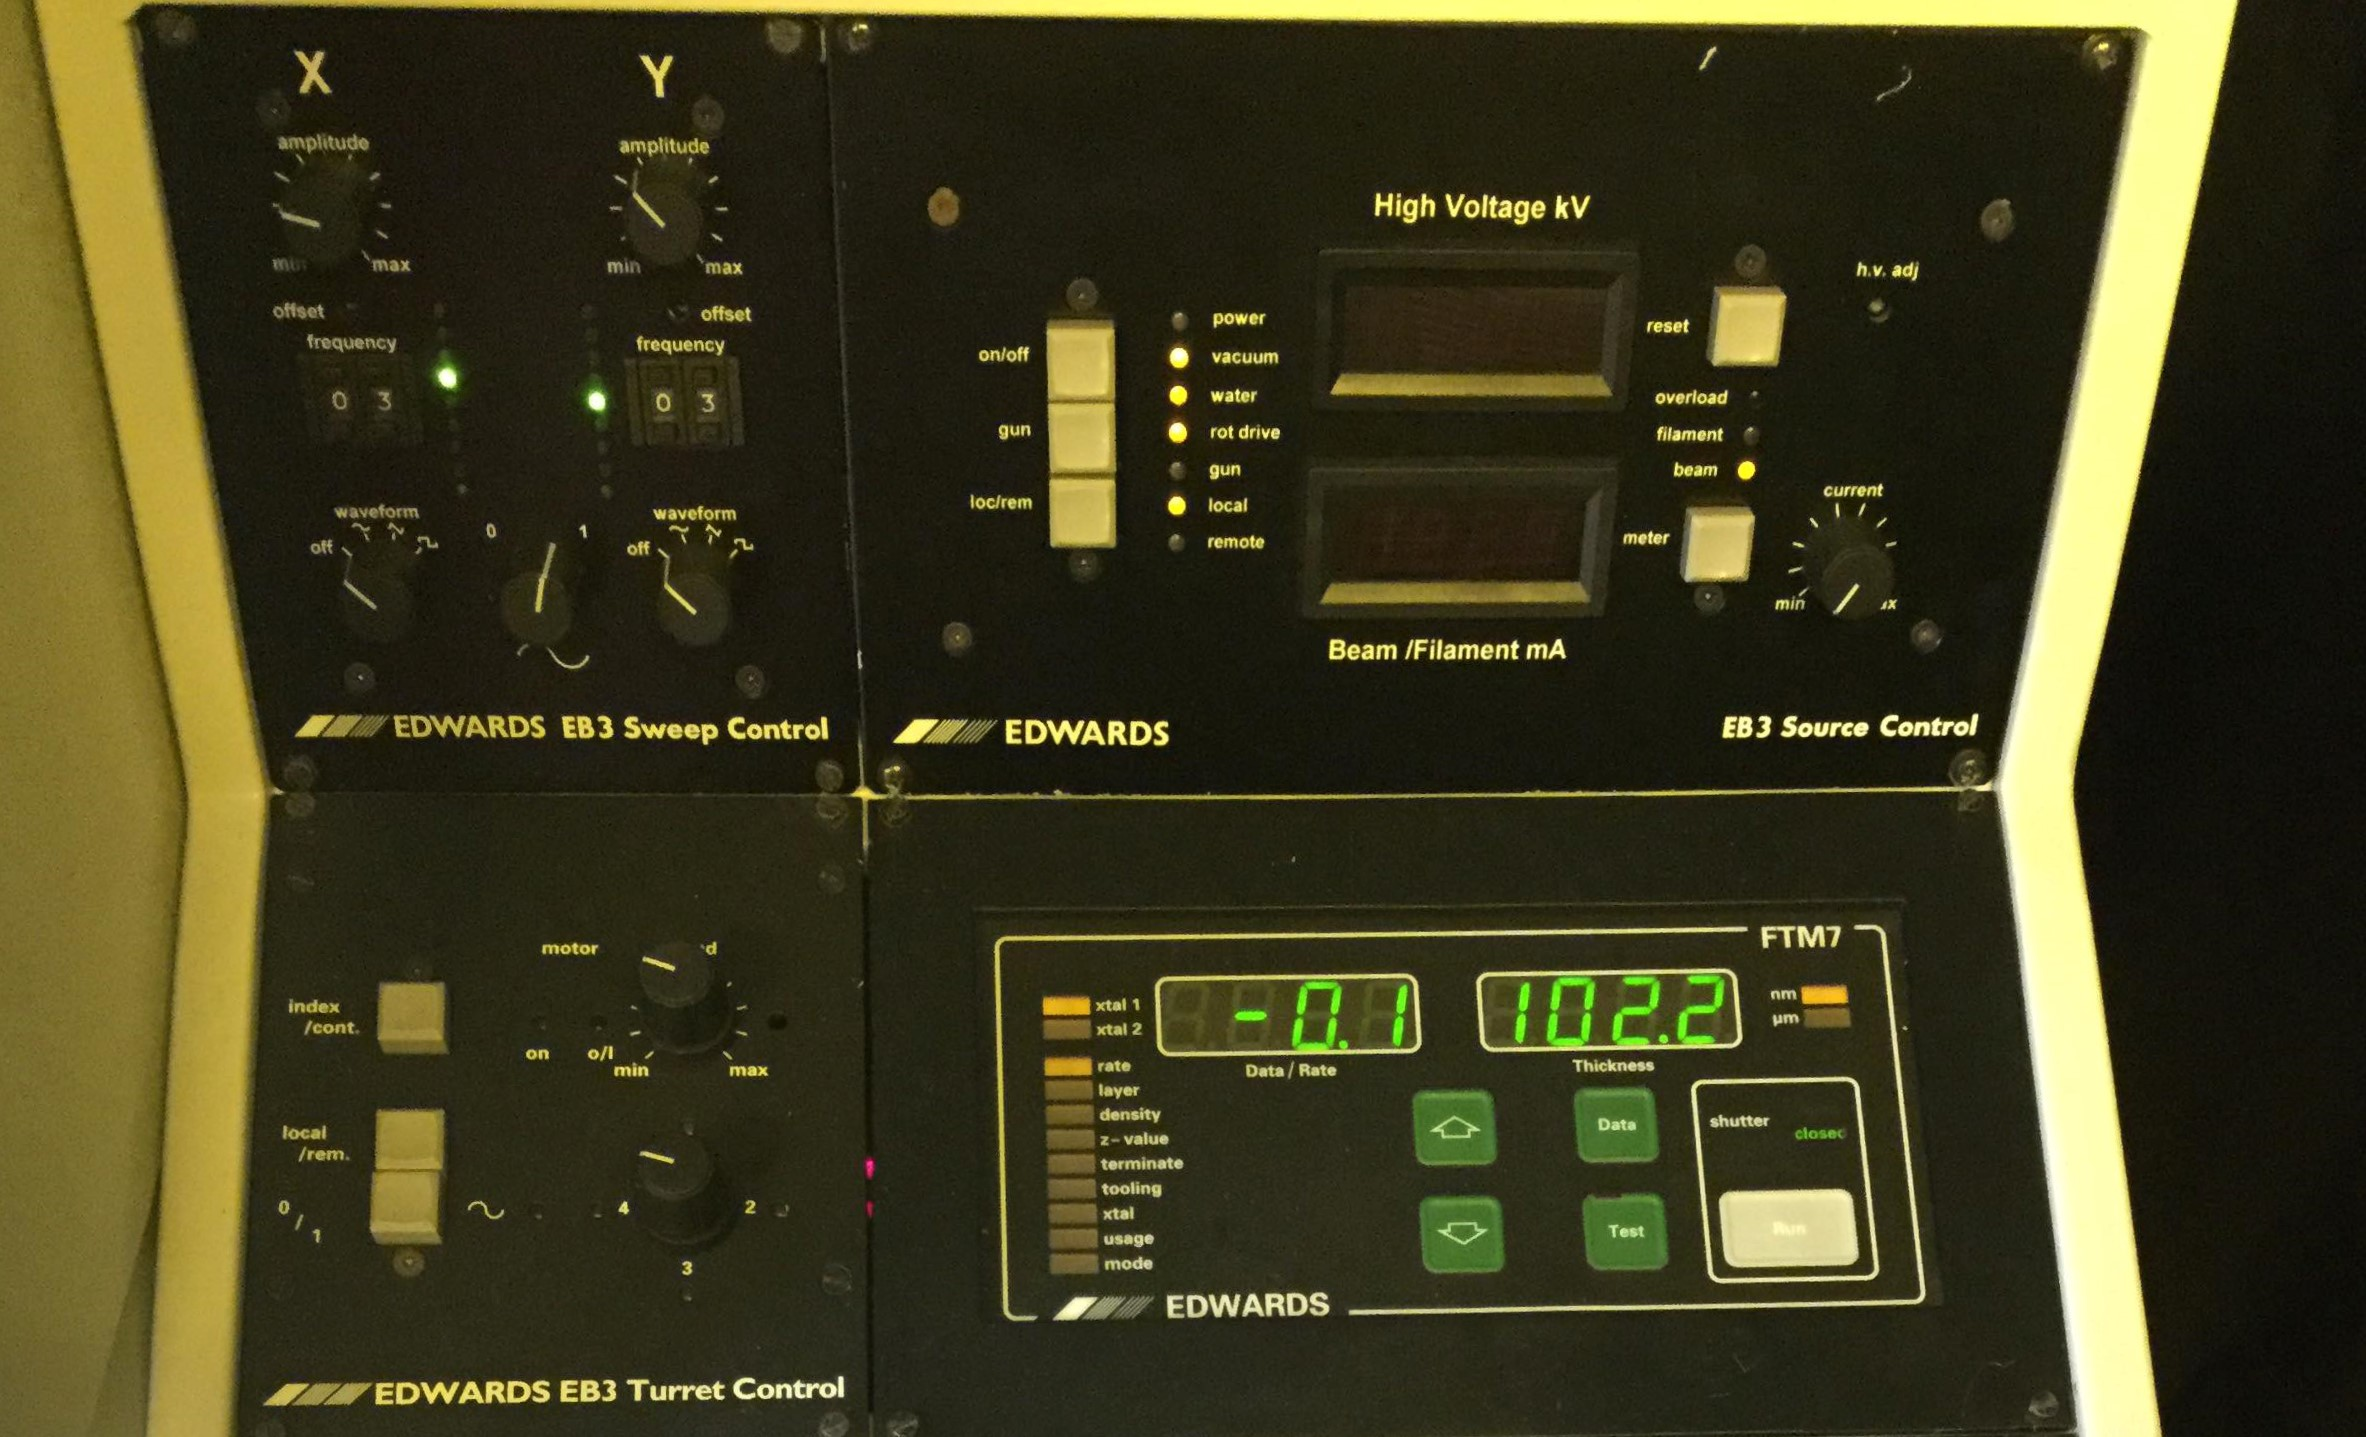
\includegraphics[width=\textwidth]{source-control}
\caption{E-Beam controls for the electron gun, sweep, crystal monitor, and crucible select}
\label{fig:source-control}
\end{figure}

Once the current has reached around 17 mA, the sweep control can be turned on by switching the dial from 0 to 1.
The current can then be continued to increase until the Data/Rate of the crystal monitor is a steady 0.1-0.2 nm/min.
Once the deposition has stabilized, the shutter can be opened by pressing run on the FTM7 control panel.
This will automatically open the shutter until the predefined thickness, usually around 100nm, is reached.
The shutter will then automatically close and the current can slowly be reduced to zero.

\begin{sidewaysfigure}
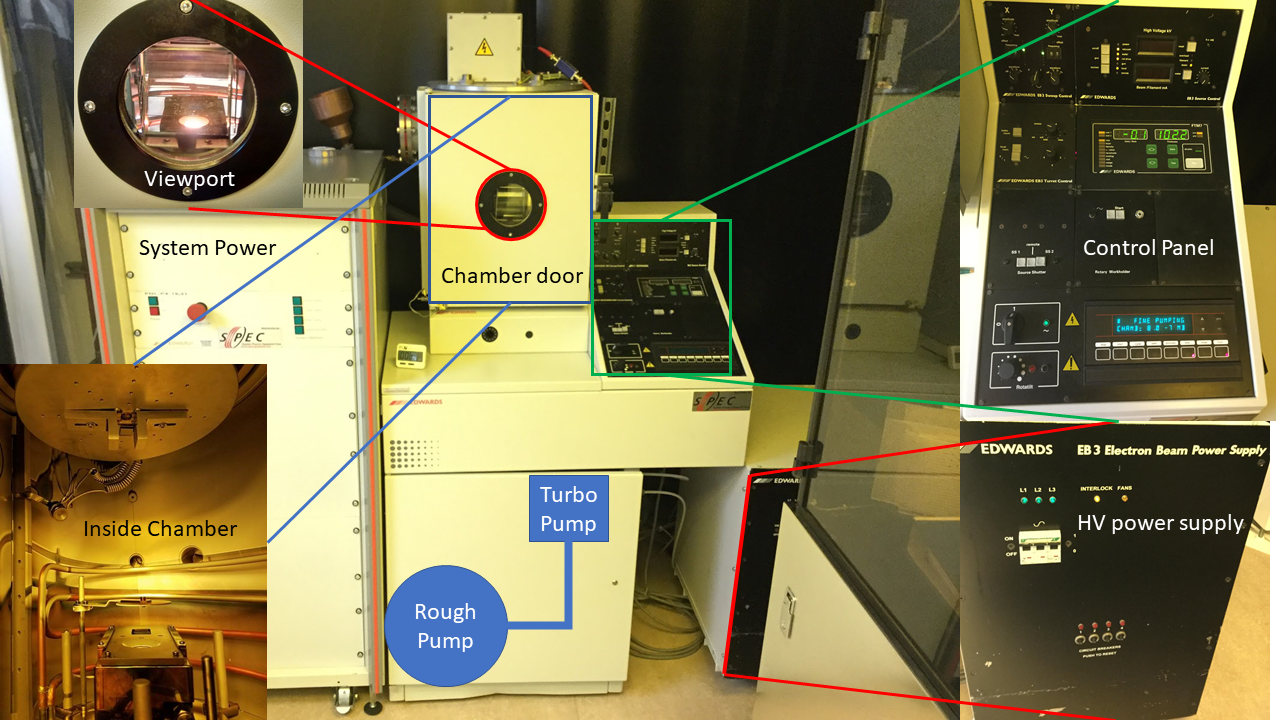
\includegraphics[width=\textwidth]{ebeam-flow}
\caption{This is a diagram of the of the electron beam machine.It is used to deposit aluminum onto the detector sample.}
\label{fig:ebeam-flow}
\end{sidewaysfigure}

\section{Final Steps}
The nature of e-beam deposition usually leaves the entire chamber coated with aluminum, including the side surface of the detector sample.
While aluminum is great for the contacts, it can cause the detector to breakdown if any is left on the surfaces other than the contacts.
Thus after aluminum deposition, the sides must be etched with acid to remove any aluminum before the detector can be tested.
However, this etch must not attack any of the aluminum left over on the surface.
To prevent this from happening, a mask of tape is placed over the top and bottom surfaces before etching as seen in Figure \ref{fig:taped}.
The tape used is acid resistant and has low adhesion so that the surface will not be damaged and no residue will be left after it is removed.
\begin{figure}[htpb]
\centering
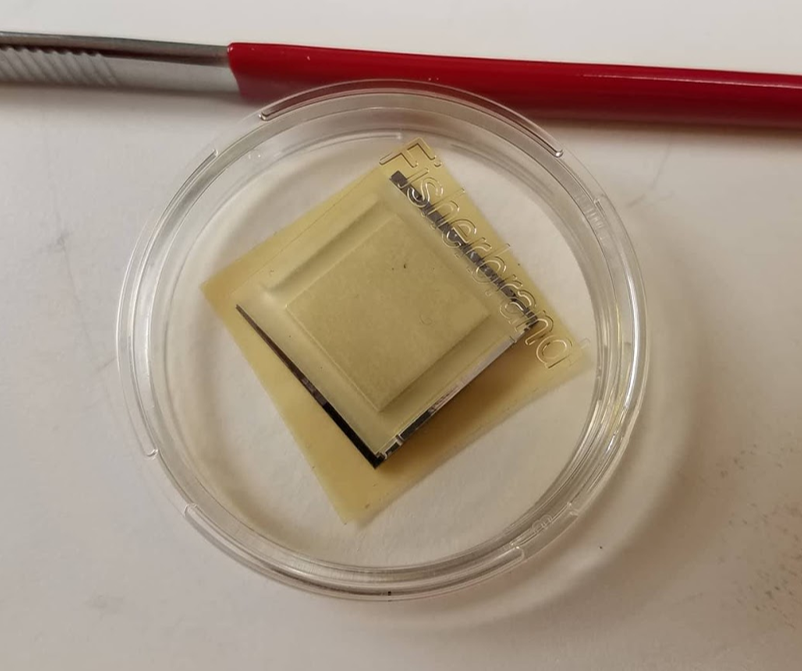
\includegraphics[width=0.5\textwidth]{taped}
\caption{Detector with tape masking before etching.}
\label{fig:taped}
\end{figure}

The taped sample is dipped in 1\% HF for a few minutes until all of the aluminum has been etched away.
The HF does not attack germanium so the AGe blocking layer beneath will be untouched.
After the aluminum is etched away, the tape is carefully removed using a Q-tip and tweezer being careful to not scratch the surface.
The detector is now complete and can be loaded into the cryostat for testing.



